%\chapter{Introduction générale} \label{Introduction générale}
\setcounter{section}{0} % 
\renewcommand*{\theHsection}{chY.\the\value{section}}
% COVER PAGE
\centerline{\bfseries\textcolor{bleusection}{ \Huge Méthodologie}}  

\bigskip

% Figure cover
\begin{tikzpicture}
  \def\ig{%
   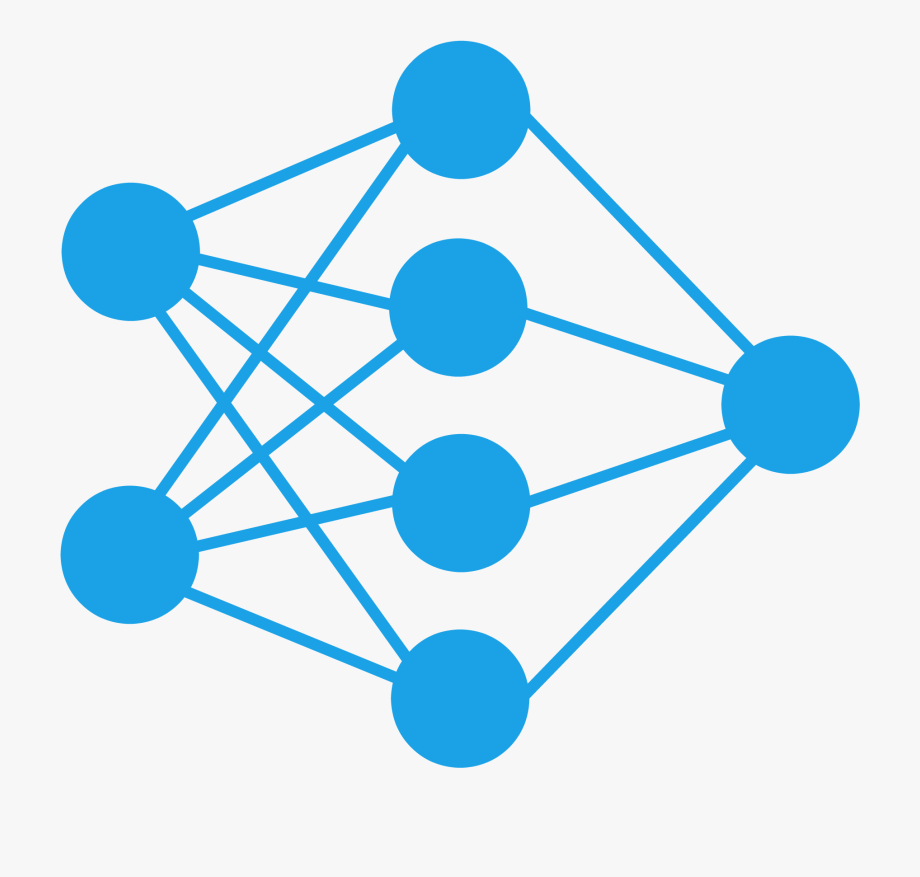
\includegraphics[width=\linewidth,keepaspectratio]{./2_methodologie/cover}}
 \node [inner sep=0pt](mypicture) at (0,0) {\phantom{\ig}};
 \clip[rounded corners=5mm] ($(mypicture.south west)+(\bord,\bord)$) rectangle ($(mypicture.north east)-(\bord,\bord)$);
 \node[inner sep=0pt](mypicture) at (0,0) {\ig};
\end{tikzpicture}

% Table des matières méthodes
{\LARGE
\begin{enumerate}[label=\textcolor{bleusection}{\arabic*}{.}, leftmargin=2cm]
  \item \nameref{methodes.1}
  \item \nameref{methodes.2}
\end{enumerate}
}

% DEBUT METHOGOLOGIE
\clearpage
\pagestyle{methodo}

\section[Analyses d'images]{Analyses d'images par apprentissage profond}\label{methodes.1}
\subsection{Historique des réseaux de neurones convolutifs}
\subsubsection{Du neurone au réseau de neurones}
\subsubsection{Analyses d'images: les convolutions}
\subsubsection{Vers des réseaux de plus en plus profonds}

\newpage

\subsection[Reconnaissance d'espèces]{Application pour la reconnaissance d'espèces}
\subsubsection{Des données généralement complexes et bruitées}
\subsubsection{Stratégies d'optimisation des performances}
\subsubsection{Reconnaissance d'espèces de corail: un cas d'étude complexe}

\newpage

\section[La photogrammétrie sous marine]{La photogrammétrie sous marine : principes et contraintes}\label{methodes.2}
\subsection{La photogrammétrie}
\subsubsection{Principes théoriques}
\subsubsection{Acquisition des images}
\subsubsection{Résolution et précision des modèles}

\newpage

\subsection{Spécificités du milieu marin}
\subsubsection{Illumination naturelle variable et faible}
\subsubsection{La réfraction}
\subsubsection{Présence d'objets mobiles sur la scène}

\newpage

\subsection[Photogrammétrie et écologie marine]{Utilisation de la photogrammétrie en écologie marine}
\subsubsection{Cartographie 2D à partir d'orthomosaïques}
\subsubsection{Extraction d'informations de modèles 3D}

\newpage

